\documentclass[reqno]{article}
\usepackage{../format-doc}

\newcommand{\fb}{f_\text{bulk}}
\newcommand{\fe}{f_\text{elastic}}
\newcommand{\fs}{f_\text{surf}}
\newcommand{\tr}{\text{tr}}
\newcommand{\Tr}{\text{Tr}}
\newcommand{\n}{\hat{\mathbf{n}}}
\newcommand{\m}{\hat{\mathbf{m}}}
\newcommand{\boldl}{\hat{\mathbf{l}}}
\newcommand{\opp}{\text{opp}}
\newcommand{\adj}{\text{adj}}
\newcommand{\hyp}{\text{hyp}}

\begin{document}
\title{Q-tensor initialization notes}
\author{Lucas Myers}
\maketitle

In general, a $Q$-tensor is given by:
\begin{equation}
    Q 
    = 
    q_1 \left(\n \otimes \n\right)
    + q_2 \left(\m \otimes \m\right)
    - (q_1 + q_2) \left( \boldl \otimes \boldl \right)
\end{equation}
We want to make $q_1$ and $q_2$ to be:
\begin{align}
    q_1(r)
    &=
    \frac{q_0}{4} \left(3 \tanh(r) + 1 \right) \\
    q_2(r)
    &=
    \frac{q_0}{4} \left(-3 \tanh(r) + 1 \right)
\end{align}
This way, $q_1 \to q_0$ and $q_2 \to -q_0 / 2$ as $r \to \infty$, and $q_1 \to q_0 / 4$ and $q_2 \to q_0 / 4$.
This gives the qualitative behavior of a disclination.
For multiple disclinations, we must take the same value away from disclinations, and each disclination center must take on the same minimum value.
One way to do this is to create a function which is zero almost everywhere, and make peaks corresponding to disclination centers.
Something like $f(x) = 1 - \tanh(r)$ does such a thing.

\begin{figure}[!h]
\centering
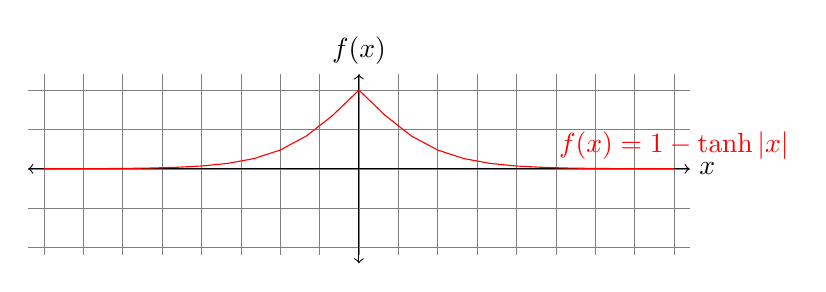
\begin{tikzpicture}[domain=-4:4]
  \draw[step=0.5cm,very thin,color=gray] (-4.2,-1.1) grid (4.2,1.2);
  \draw[<->] (-4.2,0) -- (4.2,0) node[right] {$x$};
  \draw[<->] (0,-1.2) -- (0,1.2) node[above] {$f(x)$};
  \draw[color=red] plot (\x,{1 - tanh(abs(\x))}) node[above] {$f(x) = 1 - \tanh|x|$};
\end{tikzpicture}
\end{figure}

To get back to the appropriate eigenfunctions, one must transform as $T_1(y) = (q_{1, \text{max}} - q_{1, \text{min}})(1 - y) + q_{1, \text{min}}$ and $T_2(y) = (q_{2, \text{max}} - q_{2, \text{min}}) y + q_{2, \text{min}}$.
To get multiple disclinations, you just add $y$'s at different locations.
In total, this gives:
\begin{align}
    q_1(x) 
    &= 
    (q_{1, \text{max}} - q_{1, \text{min}})\left((1 - n) + \sum_i^n \tanh r_i \right) + q_{1, \text{min}}  \\
    q_2(x)
    &=
    (q_{2, \text{max}} - q_{2, \text{min}}) \left( n - \sum_i^n \tanh r_i \right) + q_{2, \text{min}}
\end{align}
For a two-dimensional director system, we may just add up the different director angles of isolated disclinations to get the entire configuration director angle.
For a $2D$ system whose plane is defined by the $z$-axis, the director is given by:
\begin{equation}
    \n
    =
    \begin{bmatrix}
        \cos\theta \\
        \sin\theta \\
        0
    \end{bmatrix}
\end{equation}
Additionally, the secondary eigenvector is given by:
\begin{equation}
    \m
    =
    \begin{bmatrix}
        -\sin\theta \\
        \cos\theta \\
        0
    \end{bmatrix}
\end{equation}
and the last eigenvector is given by:
\begin{equation}
    \boldl
    =
    \begin{bmatrix}
        0 \\
        0 \\
        1
    \end{bmatrix}
\end{equation}
For all of these, if the disclination is to be oriented along a different axis, one must just cycle the vector entries appropriately.

If we want to twist the configuration, we have to apply a rotation matrix to $\n$ and $\m$:
\begin{equation}
    R(\alpha z)
    =
    \begin{bmatrix}
        \cos(\alpha z) &-\sin(\alpha z) &0 \\
        \sin(\alpha z) &\cos(\alpha z) &0 \\
        0 &0 &1
    \end{bmatrix}
\end{equation}
Again, if we wish to have our disclinations oriented along a different axis, we must just permunte the rows and columns of this smatrix.
We note that $\alpha$ is the angular frequency that the configuration is twisted in the $z$-direction.
Hence, it undergoes a full twist in $z = 2\pi / \alpha$ distance.
Given some cylindrical cavity length $L$, the angular frequency for a single rotation is $\alpha = 2 \pi / L$.

\end{document}
